% Section content template for individual Educative lessons
% This file contains the actual content for a specific section
% Generated from Educative API section content

% Section: Activity Diagram for the Movie Ticket Booking System
% Section ID: 6345062630031360
% Section Slug: activity-diagram-for-the-movie-ticket-booking-system
% Generated: 2025-12-12T14:19:52.017924

An activity diagram is a great way to visualize the flow of messages from one activity to another in the system. There can be different activity diagrams that we can create for our movie ticket booking system. In this lesson, we will create activity diagrams for the following two activities:

\begin{itemize}
\item
\protect\phantomsection\label{Sxo-A9j6UjHliGvs06ZnY}
The customer makes a booking for the movie.
\item
\protect\phantomsection\label{ZrF2WGngDeqymvqJT4Wc_}
\textbf{Activity challenge:} The admin cancels a show.
\end{itemize}

\subsection{The customer makes a booking for the movie}\label{b97MP6UHJNsTAhQksTikt}
\\
The following are the states and actions that will be involved in this activity diagram.

\subsubsection{States}\label{85bEWEh9TMDHiHaAUWYR8}

\begin{itemize}
\item
\protect\phantomsection\label{bOZBbAzNwPjOHz3g09QTh}
\textbf{Initial state:} The customer opens a search for a movie.
\item
\protect\phantomsection\label{6MeBSZpNBZuCVqyL40LUi}
\textbf{Final state:} The customer receives a ticket for the movie.
\end{itemize}

\subsubsection{Actions}\label{TUTlraPZcIU0Gv7i6onjm}
\\
The customer searches for a movie using specific criteria and selects it. The customer then selects their required seat and pays according to the seat type. The payment is made either through cash or a credit card. After successful payment, the customer receives the movie ticket.
\\
Based on the order above, the activity diagram of a customer making a booking for the movie is given below.
\begin{quote}
\textbf{Note:} Here, we assume the customer is purchasing a single cinema seat.
\end{quote}

\begin{figure}[htbp]
 \centering
 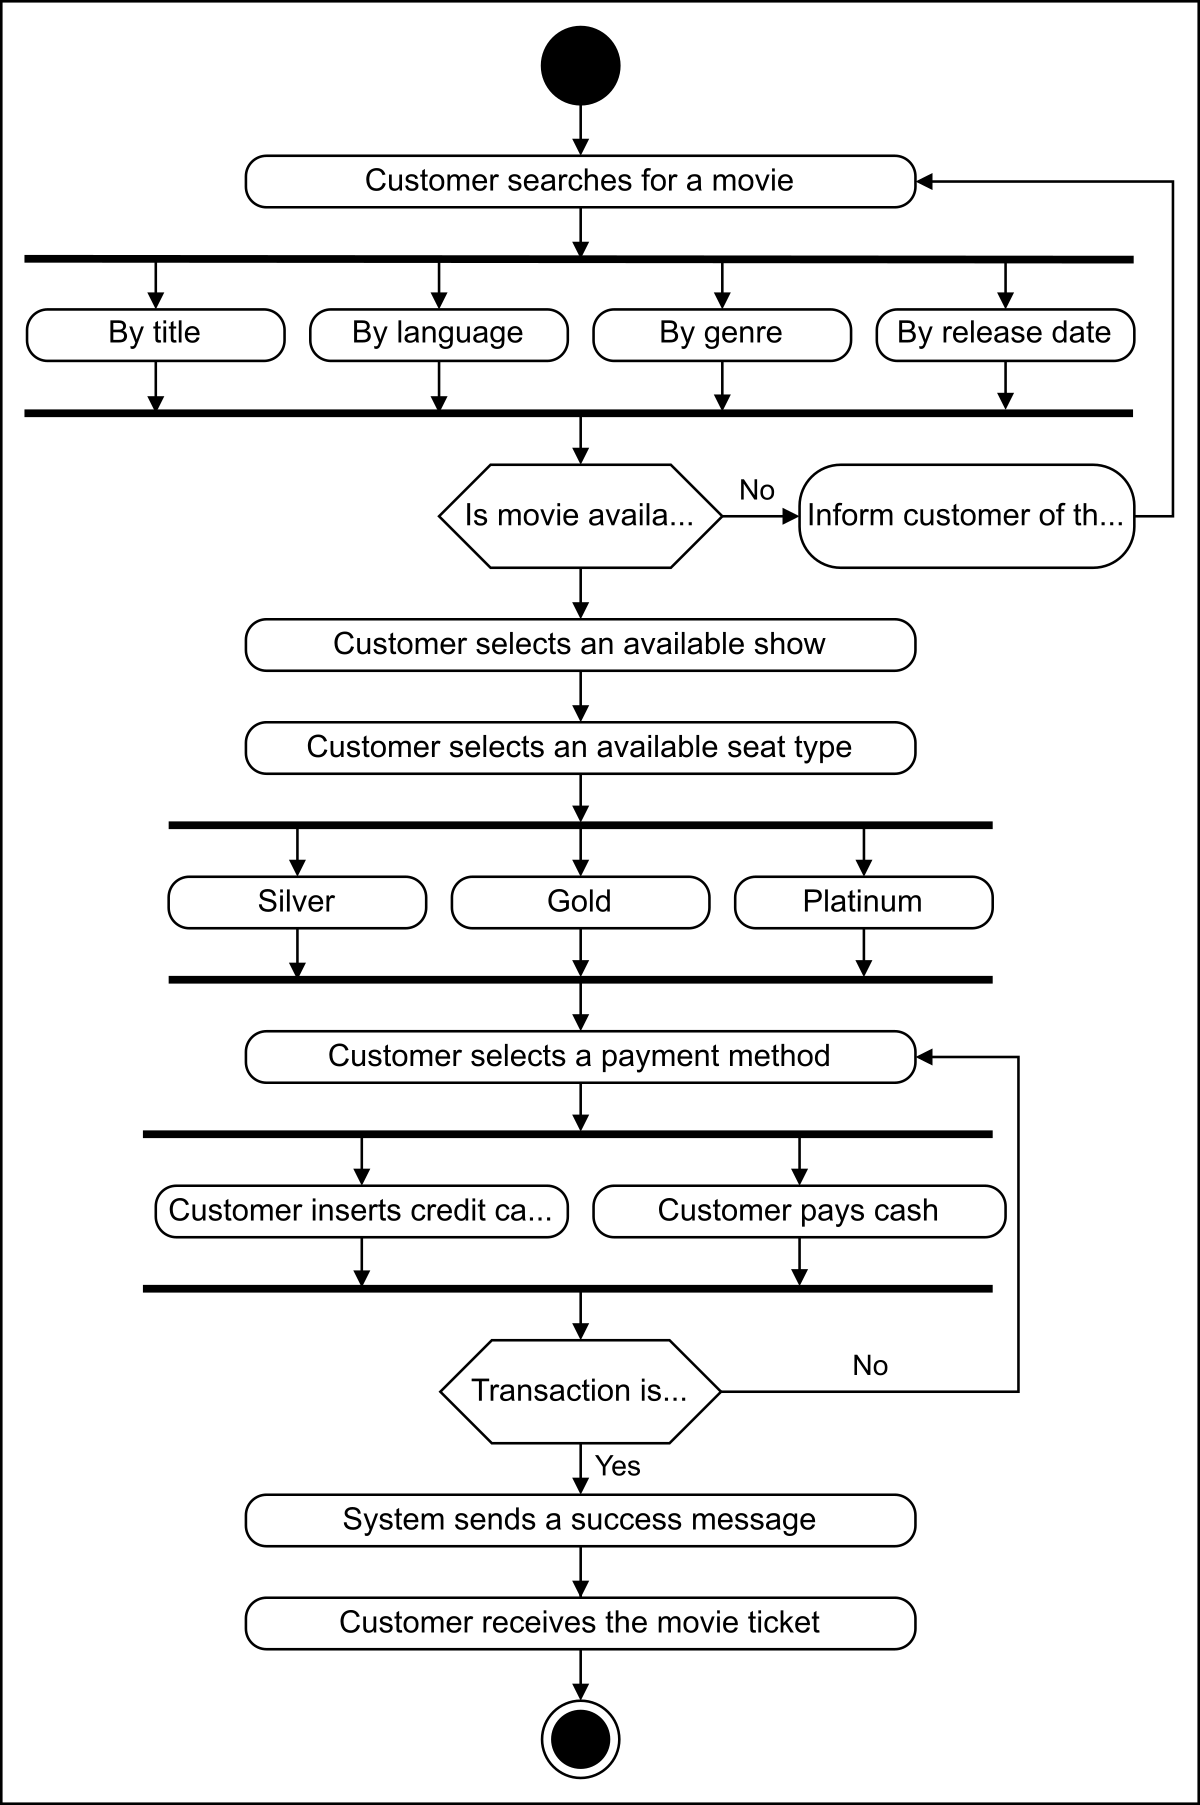
\includegraphics[width=0.5\textwidth]{Images/chapter_14/section_6345062630031360/5682179423338496.png}
 \caption{The activity diagram for the customer making a booking}
\end{figure}

\subsection{Activity challenge: Admin cancels a show}\label{qQ8UiLDWEEf6Cnibbq9TJ}
\\
You will create an activity diagram of an admin canceling a show for a movie.
\\
A skeleton of the activity diagram is given below.

\begin{figure}[htbp]
 \centering
 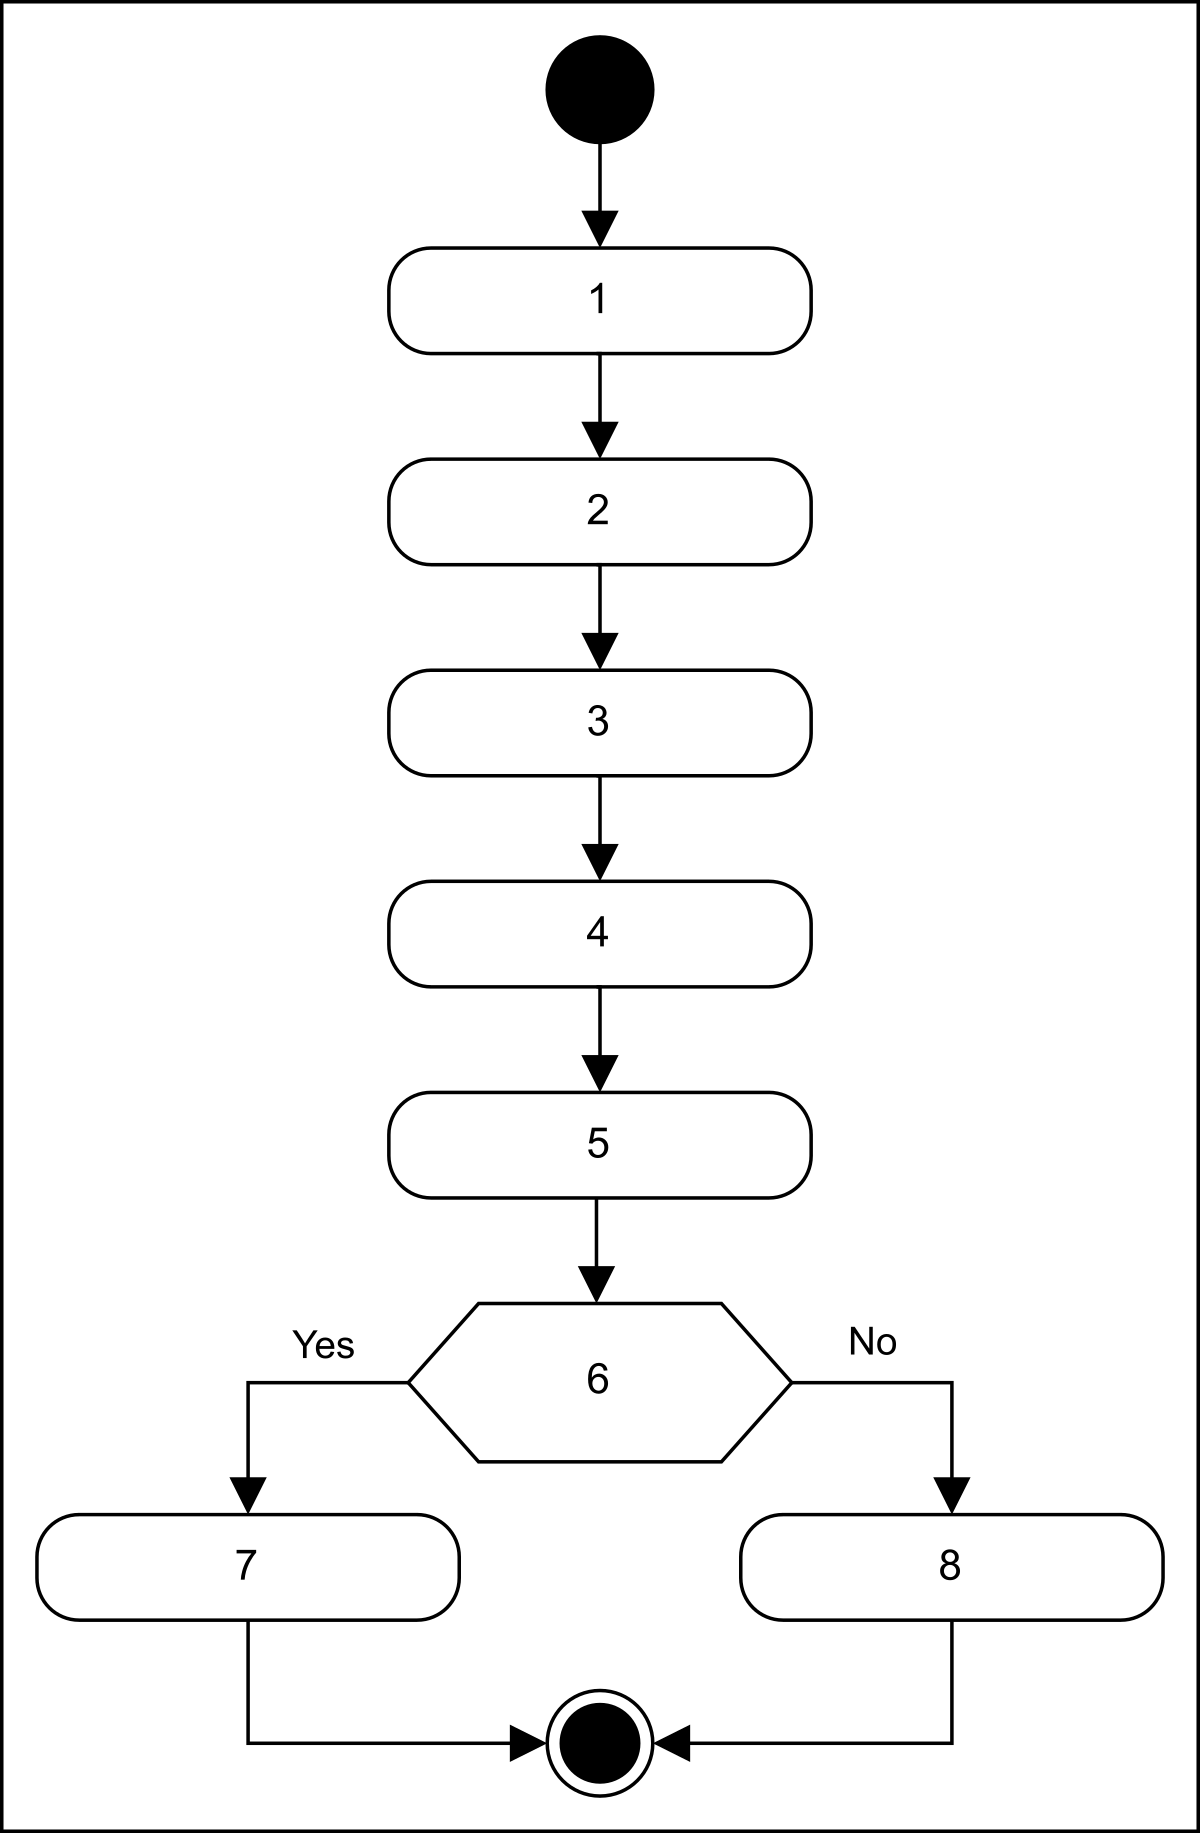
\includegraphics[width=0.5\textwidth]{Images/chapter_14/section_6345062630031360/6712827345895424.png}
 \caption{The activity diagram for an admin cancelling a show}
\end{figure}

Notice that the actions in the diagram above are numbered from 1 to 8. The slots shown below represent the activities, and the arrows represent the flow from one activity to the other.
\\
Can you rearrange the given slots in the correct order they should appear in the activity diagram above?
\begin{quote}
\textbf{Note:} If you're stuck, click the ``Show Solution'' button.
\end{quote}

Alternatively, you can also click the ``Show complete diagram'' button below to see the complete sequence diagram.

We've looked at some of the activity diagrams of our movie ticket booking system. In the next lesson, we will present the code for our designed classes in some of the most popular languages.

% End of section content